\documentclass[10pt, compress]{beamer}

\usetheme{m}

\usepackage{graphicx}
\usepackage{booktabs}
\usepackage[scale=2]{ccicons}
\usepackage{minted}
\usemintedstyle{perldoc}

\usepgfplotslibrary{dateplot}

\usemintedstyle{trac}

\usepackage{datetime}
\newdate{date}{03}{08}{2015}

\usepackage{verbatim}
\usepackage{tikz}
%\usetikzlibrary{shapes.geometric, arrows}
\usetikzlibrary{shapes,arrows,shadows}
\tikzstyle{startstop} = [rectangle, rounded corners, minimum width=3cm, minimum height=1cm,text centered, draw=black, fill=red!30]
\tikzstyle{io} = [ellipse, minimum width=3cm, minimum height=1cm, text centered, draw=black, fill=blue!30]
\tikzstyle{arrow} = [thick,->,>=stealth]

\title{Advanced Quantitative Methods Clinic}
\subtitle{Master’s in Sustainability Leadership,\\
Cambridge Institute for Sustainability Leadership}
\date{\displaydate{date}}
\author{Sreekumar Thaithara Balan}
\institute{Department of Physics and Astronomy,\\
University College London}

\begin{document}

\maketitle

%
\section{Outline}

\begin{frame}
    \frametitle{Outline}
    \begin{itemize}
        \item Software for data analysis ($\sim$15mins)
        \item Data visualisation ($\sim$20mins)
        \item Descriptive statistics ($\sim$20mins)
        \item Inferential statistics ($\sim$20mins)
        \item Regression ($\sim$20mins)
        \item Discussion ($\sim$10mins)
    \end{itemize}
\end{frame}

\section{Software for data analysis}

\begin{frame}[fragile]
    \frametitle{Software for data analysis}
    A large list can be found in \href{https://en.wikipedia.org/wiki/List_of_statistical_packages}{\texttt{Wikipedia}}.
    Some widely used ones are below.
    \begin{itemize}
        \item \texttt{Python}, \url{https://www.python.org/} %{\texttt{Python}}
        \item \texttt{R}, \url{https://cran.r-project.org/}%{\texttt{R}}
        \item \texttt{Excel}, \url{https://products.office.com/en-us/excel}%{\texttt{Excel}}
    \end{itemize}
    I will demostrate the examples using \texttt{Python}. If you have no prior
    experience, no problem, there will be plenty of help.
\end{frame}

\begin{frame}[fragile]
    \frametitle{Software set-up}
    We need at least one of the statistical softwares mentioned in the
    previous slide. Please follow the instructions below
    \begin{itemize}
        \item \url{http://docs.continuum.io/anaconda/install}%{\texttt{Python}}
        \item \url{https://cran.r-project.org/}%{\texttt{R}}
        \item \url{https://products.office.com/en-us/excel}%{\texttt{Excel}}
    \end{itemize}
    \smallskip
    \alert{Has everyone installed one of the above?}
\end{frame}

\section{Data visualisation}

\begin{frame}
    \frametitle{Data visualisation}
    \begin{columns}
        \column{0.5\textwidth}
        \begin{block}{examples}
            \begin{itemize}
                \item{bar-charts}
                \item{histograms}
                \item{scatter-plots}
                \item{errobars}
                \item{pie-charts}
                \item{many more!}
            \end{itemize}
        \end{block}
        %
        \column{0.5\textwidth}
        \begin{block}{}
            %\alert{\huge A picture is worth a thousand words}
            \begin{figure}
                \begin{center}
                    \includegraphics[scale=0.2]{img/121236_NewPieCharts720.png}
                    %http://map.gsfc.nasa.gov/universe/uni_matter.html
                \end{center}
            \end{figure}
        \end{block}
        %
    \end{columns}
\end{frame}

\begin{frame}
    \frametitle{Data visualisation: Examples}
    \begin{itemize}
        \item We have several examples in the repository.
        \item Please follow the instructions in \url{https://github.com/tbs1980/CISLQuantWorkshop/tree/master/AdvancedQuantitativeMethodsClinic}.
        \item Try to finish the first example.
        \item We have 15 mins for this session.
        \item Get your hands dirty!
    \end{itemize}
\end{frame}

\section{Descriptive statistics}

\begin{frame}
    \frametitle{Descriptive statistics}
    \begin{itemize}
        \item Definitions
        \item Freqency distributions
        \item Central tendency and variability
    \end{itemize}
\end{frame}

\begin{frame}
    \frametitle{Definitions}
    \begin{columns}
        \column{0.5\textwidth}
        \begin{block}{Glossary}
            \begin{itemize}
                \item Population
                \item Samples
                \item Variable
                \item Data
                \item Parameter
                \item Statistic
            \end{itemize}
        \end{block}
        %
        \column{0.5\textwidth}
        \begin{block}{}
            \begin{figure}
                \begin{center}
                    \includegraphics[scale=0.7]{img/as1-10-popvsam.png}
                    %http://ihsmath11.wikispaces.com/AS1.10+Population+vSample
                \end{center}
            \end{figure}
        \end{block}
    \end{columns}
\end{frame}

%
% TODO MORE SLIDES ON THE DEFINITIONS
%

\begin{frame}
    \frametitle{Freqency distributions}
    \begin{columns}
        \column{0.5\textwidth}
        \begin{block}{Defined by}
            \begin{itemize}
                \item Size
                \item Range
                \item Bins-size
                \item Normalisation
            \end{itemize}
        \end{block}
        %
        \column{0.5\textwidth}
        \begin{block}{}
            \begin{figure}
                \begin{center}
                    \includegraphics[scale=0.3]{img/hist_new_stacked.png}
                    %http://pandas.pydata.org/pandas-docs/stable/visualization.html
                \end{center}
            \end{figure}
        \end{block}
    \end{columns}
\end{frame}

\begin{frame}
    \frametitle{Central tendency}
    \begin{columns}
        \column{0.5\textwidth}
        \begin{block}{How to characterise a distribution?}
            \begin{itemize}
                \item \alert{What is a measure of central tendency?}
                \item Mean, median and mode
            \end{itemize}
            \smallskip
            The mean $\mu$ of samples $\{x_1,x_2,\cdots,x_n\}$ can be computed
            as
            \begin{equation}
                \mu = \frac{\sum_i x_i}{\sum_i}
            \end{equation}
        \end{block}
        %
        \column{0.5\textwidth}
        \begin{block}{}
            \begin{figure}
                \begin{center}
                    \includegraphics[scale=0.5]{img/central_tendancy.jpg}
                    %http://flowjo.typepad.com/the_daily_dongle/science/
                \end{center}
            \end{figure}
        \end{block}
    \end{columns}
\end{frame}

\begin{frame}
    \frametitle{Variability}
    \begin{columns}
        \column{0.5\textwidth}
        \begin{block}{How to measure variations?}
            \begin{itemize}
                \item \alert{Are you a good shooter?}
                \item Vairance and standard deviation
                \item Population and samples
            \end{itemize}
            \smallskip
            The (biased) samples variance is defined as
            \begin{equation}
                \sigma^2 = \frac{\sum_i (x_i - \mu)^2}{\sum_i}
            \end{equation}
        \end{block}
        %
        \column{0.5\textwidth}
        \begin{block}{}
            \begin{figure}
                \begin{center}
                    \includegraphics[scale=0.4]{img/std_dvn.png}
                    %http://www.itrcweb.org/ism-1/4_3_1_3_Relative_standard_deviation_of_replicate_samples.html
                \end{center}
            \end{figure}
        \end{block}
    \end{columns}
\end{frame}

\begin{frame}
    \frametitle{Examples/Discussion}
    \begin{itemize}
        \item Examples can be found at \url{https://github.com/tbs1980/CISLQuantWorkshop/tree/master/AdvancedQuantitativeMethodsClinic/examples}
        \item Use the rest of the time for examples/discussion.
    \end{itemize}
\end{frame}

\section{Inferential statistics}

\begin{frame}
    \frametitle{Inferential statistics}
    \begin{itemize}
        \item Probability
        \item The Normal distribution
        \item Sample means and their distribution
        \item Introduction to hypothesis testing
    \end{itemize}
\end{frame}

\begin{frame}
    \frametitle{Probability}
    \begin{columns}
        \column{0.5\textwidth}
        \begin{block}{Frequency or degree of belief?}
            \begin{itemize}
                \item Frequency
                \item Desired outcome
                \item Random sample
            \end{itemize}
        \end{block}
        %
        \column{0.5\textwidth}
        \begin{block}{}
            \begin{figure}
                \begin{center}
                    \includegraphics[scale=0.2]{img/GRE_Probability.png}
                    %http://www.brightlinkprep.com/wp-content/uploads/2013/04/GRE_Probability.png
                \end{center}
            \end{figure}
        \end{block}
    \end{columns}
\end{frame}


\begin{frame}
    \frametitle{Role of Probability}
    \begin{columns}
        \column{0.5\textwidth}
        \begin{itemize}
            \item What kind of samples are likeliy to obtained from the population?
            \item What can we say about the population given a sample?
        \end{itemize}
        \column{0.5\textwidth}
        \begin{figure}
            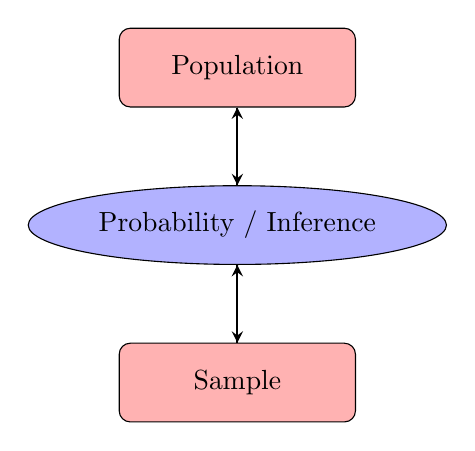
\begin{tikzpicture}[node distance=2cm]
                \node (pop) [startstop] {Population};
                \node (prob) [io,below of= pop] {Probability / Inference};
                \node (samp) [startstop,below of= prob] {Sample};
                \draw [arrow] (pop) -- (prob);
                \draw [arrow] (prob) -- (samp);
                \draw [arrow] (samp) -- (prob);
                \draw [arrow] (prob) -- (pop);
            \end{tikzpicture}
        \end{figure}
    \end{columns}
\end{frame}


\begin{frame}
    \frametitle{The Normal distribution}
    \begin{columns}
        \column{0.5\textwidth}
        \begin{block}{Characteristics}
            \begin{itemize}
                \item Mean $\mu$
                \item Standard deviation $\sigma$
                \item \alert{Why is it important?}
                \item Distribution of sample means
            \end{itemize}
            \smallskip
            \begin{equation}
                \Pr(x|\mu,\sigma)  = \frac{1}{\sigma\sqrt{2\pi}}
                    \exp\left(-\frac{1}{2}\frac{(x-\mu)^2}{\sigma^2}\right)
            \end{equation}
        \end{block}
        %
        \column{0.5\textwidth}
        \begin{block}{}
            \begin{figure}
                \begin{center}
                    \includegraphics[scale=0.4]{img/normal-curve.png}
                    %http://www.had2know.com/academics/normal-distribution-probability-calculator.html
                \end{center}
            \end{figure}
        \end{block}
    \end{columns}
\end{frame}

\begin{frame}
    \frametitle{Sample means and their distribution}
    \begin{columns}
        \column{0.5\textwidth}
        \begin{block}{Characteristics}
            \begin{itemize}

                \item Sampling error
                \item Distribution of sample means
                \item Expected value
                \item Standard error
                \item Law of large numbers
            \end{itemize}
        \end{block}
        %
        \column{0.5\textwidth}
        \begin{block}{}
            \begin{figure}
                \begin{center}
                    \includegraphics[scale=0.3]{img/14_diag_b.png}
                    %https://epilab.ich.ucl.ac.uk/coursematerial/statistics/inference/standard_error.html
                \end{center}
            \end{figure}
        \end{block}
    \end{columns}
\end{frame}

\begin{frame}
    \frametitle{Hypothesis testing}
    \begin{columns}
        \column{0.5\textwidth}
        \begin{block}{Baic idea}
            \begin{itemize}
                \item Known versus unknown
                \item Null versus alternative hypothesis
                \item Decision crieteria
                \item Level of significance
                \item Critical region
                \item Uncertanity and errors
                \item Statistical significance
            \end{itemize}
        \end{block}
        %
        \column{0.5\textwidth}
        \begin{block}{}
            \begin{figure}
                \begin{center}
                    \includegraphics[scale=0.3]{img/IQ_Hypoth.png}
                    %http://simon.cs.vt.edu/SoSci/converted/Hypoth_I/
                \end{center}
            \end{figure}
        \end{block}
    \end{columns}
\end{frame}

\begin{frame}
    \frametitle{Logic behind hypothesis testing}
    \begin{columns}
        \column{0.5\textwidth}
        \begin{block}{Questions}
            \begin{itemize}
                \item Can we observe meaningful patterns in the data
                \item Are the findings statistically significant?
                \item Does the model adeqately describe the data?
                \item Is there evidence for an alternative hypothesis?
            \end{itemize}
        \end{block}
        %
        \column{0.5\textwidth}
        \begin{block}{}
            \begin{figure}
                \scalebox{0.7}
                {
                    \begin{tikzpicture}
                        \def \n {2}
                        \def \radius {3cm}
                        \def \margin {6}
                        \def \s {1}
                        \node[draw, circle] at ({360/\n * (\s - 1)}:\radius) {Model};
                            \draw[->, >=latex] ({360/\n * (\s - 1)+\margin}:\radius)
                                arc ({360/\n * (\s - 1)+\margin}:{360/\n * (\s)-\margin}:\radius);
                        \def \s {2}
                        \node[draw, circle] at ({360/\n * (\s - 1)}:\radius) {Data};
                            \draw[->, >=latex] ({360/\n * (\s - 1)+\margin}:\radius)
                                arc ({360/\n * (\s - 1)+\margin}:{360/\n * (\s)-\margin}:\radius);
                    \end{tikzpicture}
                }
            \end{figure}
        \end{block}
    \end{columns}
\end{frame}

\begin{frame}
    \frametitle{hypothesis testing by comparing distributions}
    \begin{columns}
        \column{0.5\textwidth}
        \begin{block}{Questions}
            \begin{itemize}
                \item Known characterstics of a population
                \item Selected sample for research
                \item Characterstics of the sample after experiment
                \item How do they compare?
            \end{itemize}
        \end{block}
        %
        \column{0.5\textwidth}
        \begin{block}{}
            \begin{figure}
                \scalebox{0.7}
                {
                    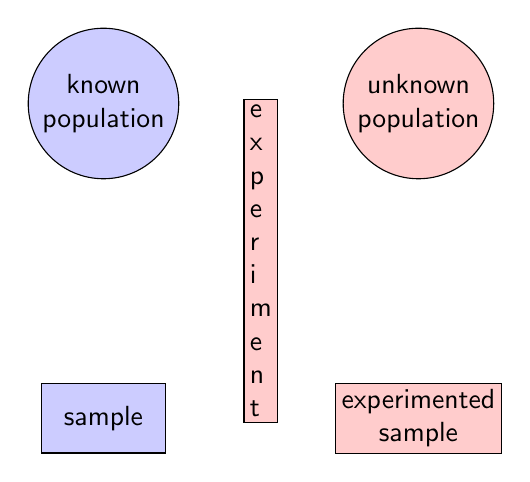
\begin{tikzpicture}
                        \node[draw, fill=red!20, rectangle, align=left,
                            inner sep=0.5ex, font=\sffamily]
                            at (0,0) { e \\ x \\ p \\ e \\ r \\ i \\ m \\ e \\ n \\ t };
                        \node[draw, fill=red!20,circle,align=center,inner sep=0.5ex,font=\sffamily]
                            at (2,2) {unknown \\ population};
                        \node[draw,fill=red!20,rectangle,align=center,inner sep=0.5ex,font=\sffamily]
                            at (2,-2) {experimented \\ sample};
                        \node[draw, fill=blue!20,circle,,align=center,inner sep=0.5ex,font=\sffamily]
                            at (-2,2) {known \\ population};
                        \node[draw,fill=blue!20,rectangle,align=center,
                            minimum height=2.5em,minimum width=4.5em,inner sep=0.5ex,font=\sffamily]
                            at (-2,-2) {sample};
                    \end{tikzpicture}
                }
            \end{figure}
        \end{block}
    \end{columns}
\end{frame}

\begin{frame}
    \frametitle{Comparing distributions statistically}
\end{frame}

\begin{frame}
    \frametitle{Examples/Discussion}
    \begin{itemize}
        \item Examples can be found at \url{blablalbla}
        \item Use the rest of the time for examples/discussion.
    \end{itemize}
\end{frame}

\section{Inferences about Population Means}

\begin{frame}
    \frametitle{Inferences about Population Means}
    \begin{itemize}
        \item $t$-statistic
        \item Analysis of Variacne (ANOVA)
    \end{itemize}
\end{frame}

\section{Regression}

\begin{frame}
    \frametitle{Regression}
    \begin{itemize}
        \item Parametric
        \item Correlation
        \item Non-parametric
    \end{itemize}
\end{frame}

\section{Discussion}

\begin{frame}
    \frametitle{Discussion and Summary}
    \begin{itemize}
        \item Descriptive and inferential statistics
        \item Hypotheis testing
        \item Regression
        \item Best practices
    \end{itemize}
\end{frame}


\end{document}
